\begin{figure}[H]
	\begin{subfigure}[t]{1\textwidth}
		\centering
		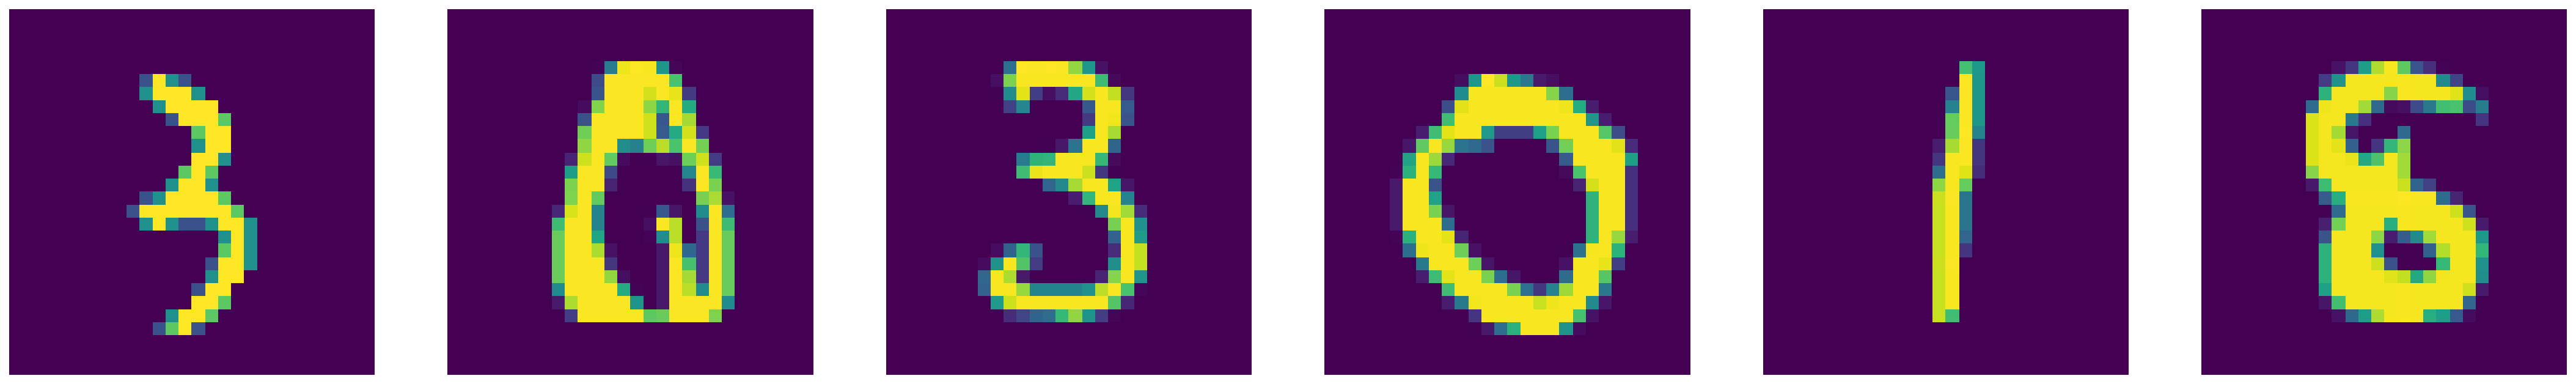
\includegraphics[width = 0.8\textwidth]{figures/ppca/real}
		\caption{Test set images}
		\label{fig:ppca:real}
	\end{subfigure}
	\begin{subfigure}[t]{1\textwidth}
		\centering
		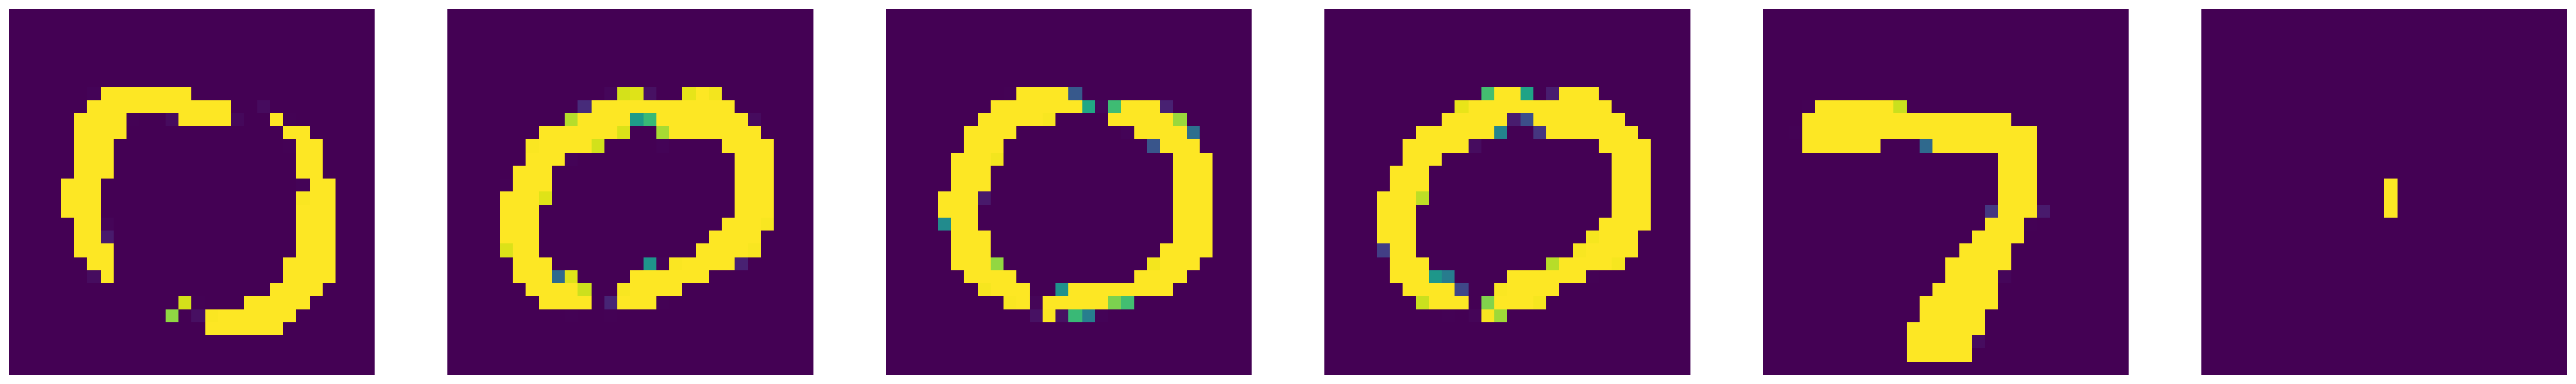
\includegraphics[width = 0.8\textwidth]{figures/vae/mean}
		\caption{VAE}
		\label{fig:ppca:mean}
	\end{subfigure}
	\begin{subfigure}[t]{1\textwidth}
		\centering
		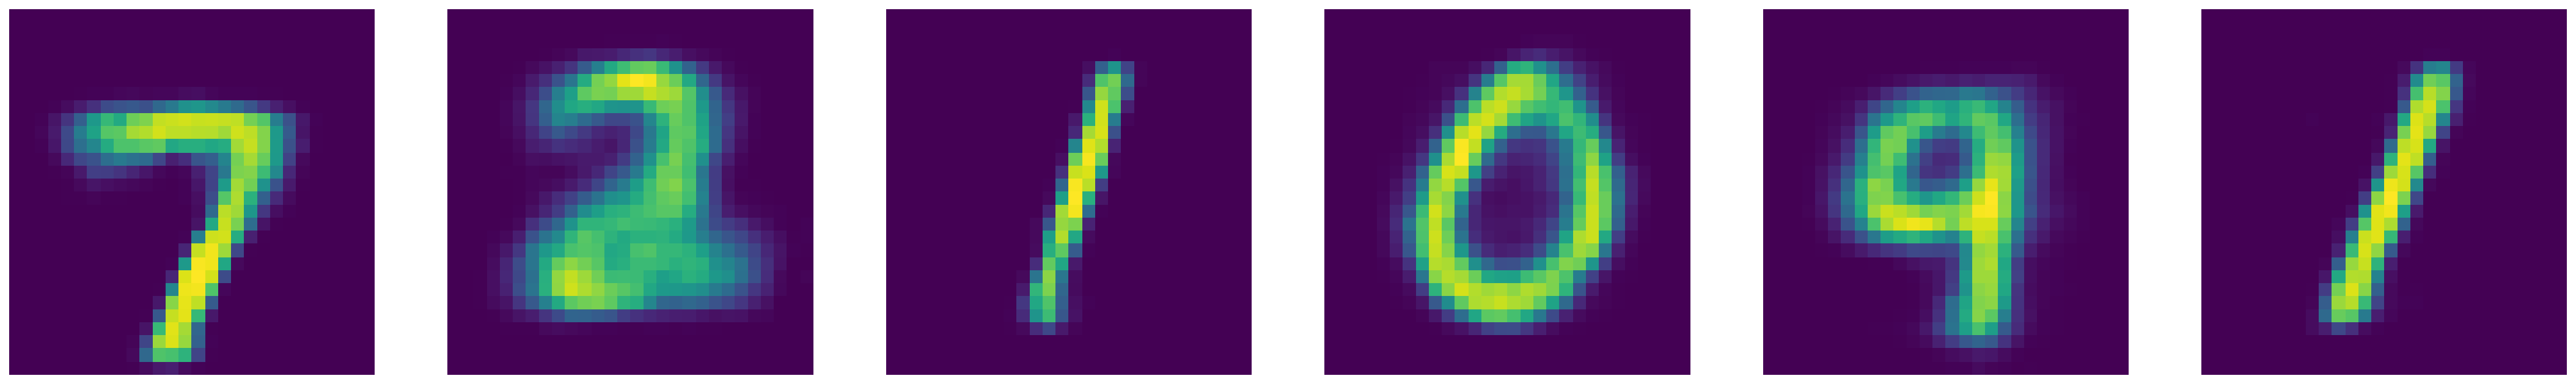
\includegraphics[width = 0.8\textwidth]{figures/cvae/mean}
		\caption{CVAE}
		\label{fig:ppca:sample}
	\end{subfigure}
	\begin{subfigure}[t]{1\textwidth}
		\centering
		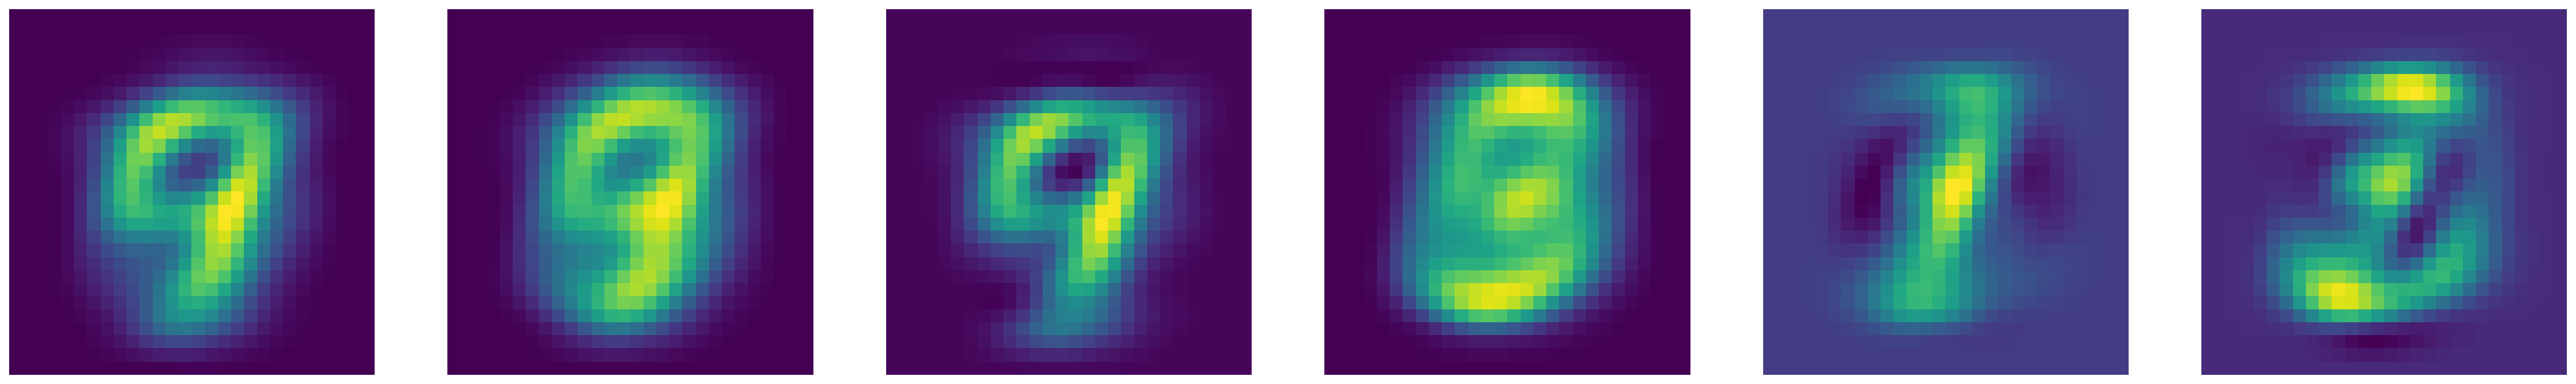
\includegraphics[width = 0.8\textwidth]{figures/ppca/mean}
		\caption{PPCA}
		\label{fig:ppca:sample}
	\end{subfigure}
	\caption{Comparison of MNIST test set images and corresponding mean parameters generated by density models}
	\label{fig:mean:_v_real}
\end{figure}


\begin{figure}[H]
	\begin{subfigure}[t]{1\textwidth}
		\centering
		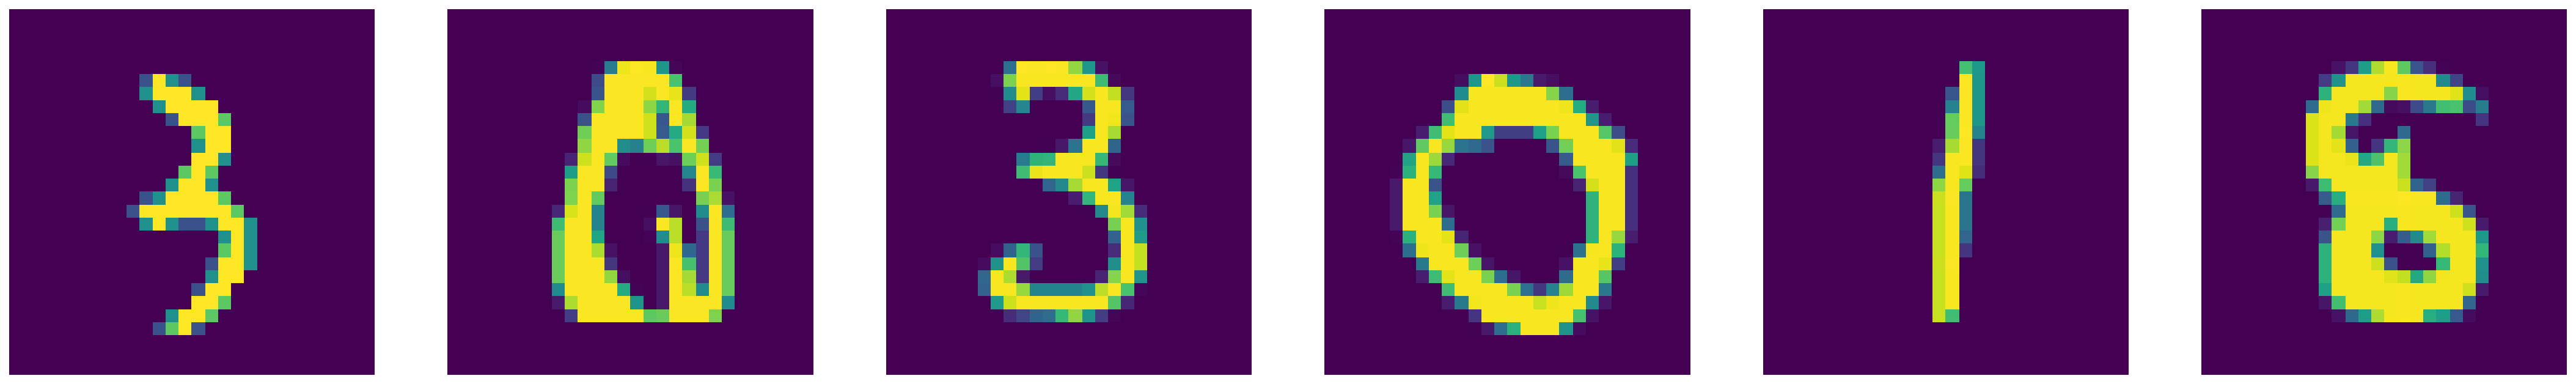
\includegraphics[width = 0.8\textwidth]{figures/ppca/real}
		\caption{Test set images}
		\label{fig:ppca:real}
	\end{subfigure}
	\begin{subfigure}[t]{1\textwidth}
		\centering
		
\includegraphics[width = 0.8\textwidth]{figures/vae/sample}
		\caption{VAE}
		\label{fig:ppca:mean}
	\end{subfigure}
	\begin{subfigure}[t]{1\textwidth}
		\centering
		
\includegraphics[width = 0.8\textwidth]{figures/cvae/sample}
		\caption{CVAE}
		\label{fig:ppca:sample}
	\end{subfigure}
	\begin{subfigure}[t]{1\textwidth}
		\centering
		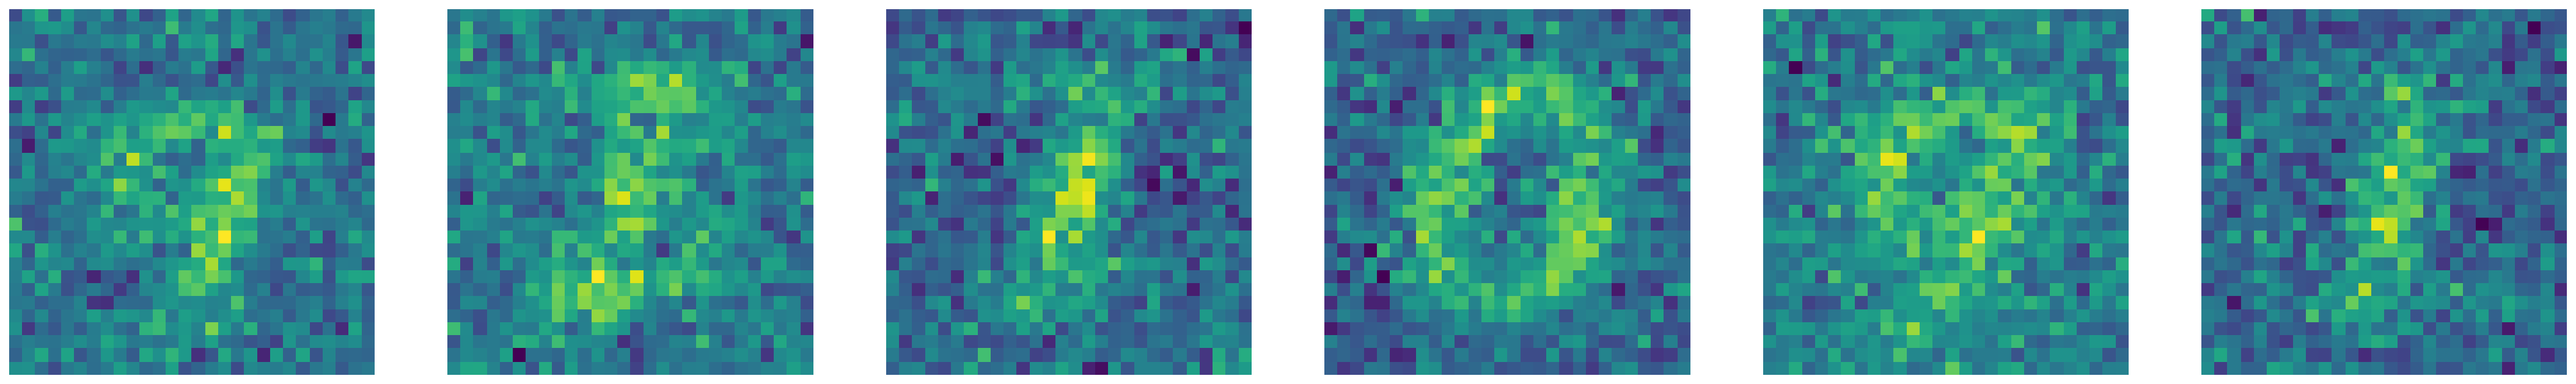
\includegraphics[width = 0.8\textwidth]{figures/ppca/sample}
		\caption{PPCA}
		\label{fig:ppca:sample}
	\end{subfigure}
	\caption{Comparison of MNIST test set images and corresponding reconstructions sampled from density models}
	\label{fig:mean:_v_real}
\end{figure}


\begin{figure}[H]
	\begin{subfigure}[t]{0.49\textwidth}
		\centering
		\includegraphics[width = 0.8\textwidth]{figures/VAE/interpolation}
		\caption{VAE}
		\label{fig:vae:interpolation}
	\end{subfigure}
	\begin{subfigure}[t]{0.49\textwidth}
		\centering
		\includegraphics[width = 0.8\textwidth]{figures/CVAE/interpolation}
		\caption{CVAE}
		\label{fig:cvae:interpolation}
	\end{subfigure}
	\begin{subfigure}[t]{0.49\textwidth}
		\centering
		\includegraphics[width = 0.8\textwidth]{figures/ppca/interpolation}
		\caption{PPCA}
		\label{fig:ppca:interpolation}
	\end{subfigure}
	\caption{Interpolating images from latent space variables using trained density models.}	
\end{figure}

\begin{figure}[H]
	\begin{subfigure}[t]{0.49\textwidth}
		\centering
		\includegraphics[width = 0.8\textwidth]{figures/VAE/clustering}
		\caption{VAE}
		\label{fig:vae:clustering}
	\end{subfigure}
	\begin{subfigure}[t]{0.49\textwidth}
		\centering
		\includegraphics[width = 0.8\textwidth]{figures/CVAE/clustering}
		\caption{CVAE}
		\label{fig:cvae:clustering}
	\end{subfigure}
	\begin{subfigure}[t]{0.49\textwidth}
		\centering
		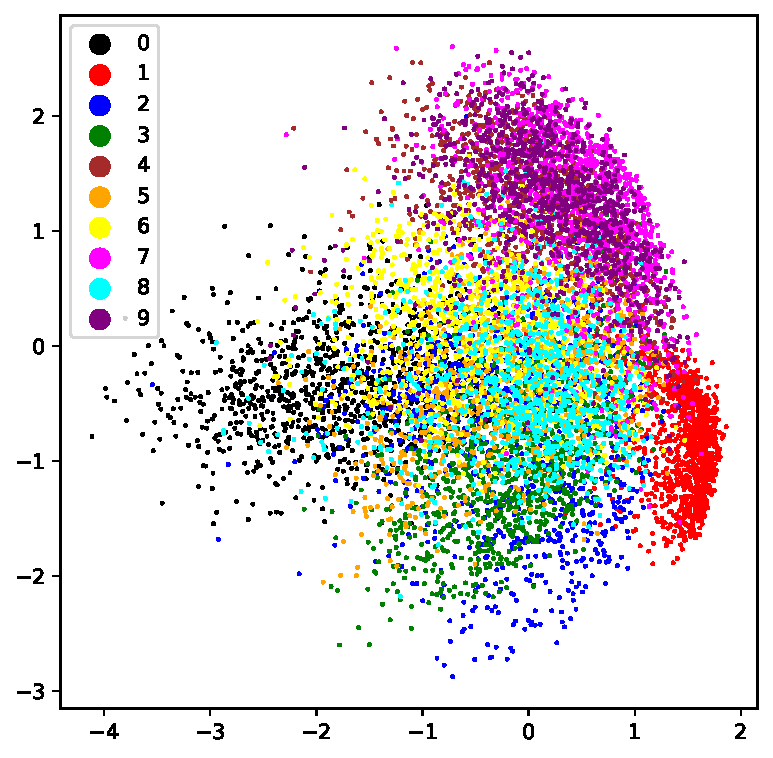
\includegraphics[width = 0.8\textwidth]{figures/ppca/clustering}
		\caption{PPCA}
		\label{fig:ppca:clustering}
	\end{subfigure}
	\caption{Clustering on MNIST test (projection to latent space) using trained density models.}	
\end{figure}

\begin{table}
\centering
\caption{Model performance metrics}
\label{table:metrics}
\begin{tabular}{ccc}
\toprule
{} &  \textbf{Log-Likelihood/ELBO} &  \textbf{MSE} \\
\midrule
\textbf{VAE } &                   -145.122048 &      0.000305 \\
\textbf{CVAE} &                   -157.241749 &      0.000352 \\
\textbf{PPCA} &                  -4329.655559 &   3620.035365 \\
\bottomrule
\end{tabular}
\end{table}
